\section{Discussion}
\label{sec:discussion}

\subsection{The embedding is the lever}
\label{sec:disc_embedding}

% --- from chapter5_embedding.tex 5.1.1-5.1.4 ---
Section~\ref{sec:results_heads} and Section~\ref{sec:results_ablation} point the same way.
The three learned heads and the ten modularity variants all add capacity or structure after the embedding,
and none improves on $k$-means once the model meets real data; in several cases, $k$-means on a head's own jointly
trained embedding does better than the head.
The failures have distinct causes: DEC sharpens its own assignments without introducing any new identity
information, slot attention carries no notion that two joints of the same type must belong to different people,
and graph partitioning turns small shifts in pairwise affinity into changes in connected components.
The modularity variants all plateau, since the $k$NN graph encodes proximity rather than identity,
and none of the ten reformulations of the objective recovered identity communities from it.
Changing the embedding, by contrast, is what produces the only gains that survive transfer --- a small one from the
three skeleton-aware modifications at matched capacity, and larger ones from the architecture sweep stacked on top
of them and from fine-tuning on COCO.
Within the grouping methods evaluated here, additional complexity at the read-out contributes less than improving the
representation it receives, and once the embedding separates people well a simple read-out is adequate.

Figure~\ref{fig:embedding} shows what this means for a single scene.
Chosen from the 180 COCO scenes with three to five people and at least ten annotated keypoints per person,
it is the one whose per-scene pose grouping accuracy under the three checkpoints lies closest to the dataset-level
accuracy, making it representative rather than chosen for effect.
The standard GATv2 embedding places several keypoints of one person inside another person's cluster, four of them
misassigned; the synthetic-only PG-GAT cuts this to three; and the fine-tuned PG-GAT collapses each person to a tight
cluster, misassigning none.
The similarity matrices show the same progression without a projection: the within-person block structure sharpens,
and cross-person similarity becomes uniform.

\begin{figure*}[!t]
    \centering
    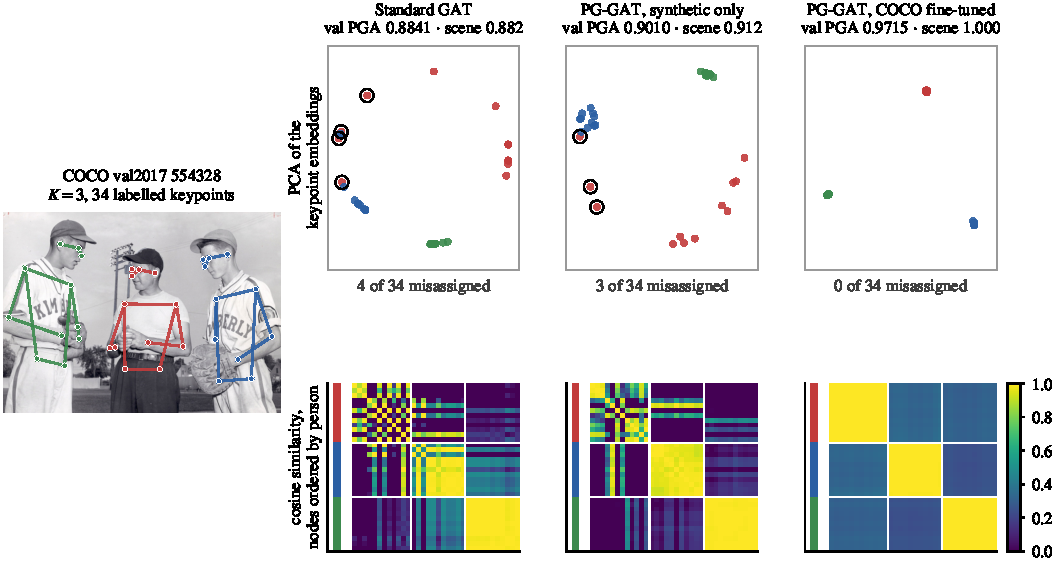
\includegraphics[width=\textwidth]{figures/embedding_space_pca.pdf}
    \caption{The embedding of one COCO \texttt{val2017} scene (554328, three people, 34 annotated keypoints) under three checkpoints: the standard GATv2 baseline, PG-GAT after synthetic training, and PG-GAT after COCO fine-tuning.
    Top: principal-component projection of the keypoint embeddings, coloured by person;
    keypoints the $k$-means read-out assigns to the wrong person are ringed.
    Bottom: cosine similarity between the keypoint embeddings, ordered by person.
    Column titles give the dataset-level pose grouping accuracy on COCO and the pose grouping accuracy on this scene.}
    \label{fig:embedding}
\end{figure*}

Where the modifications act can be read from the attention itself (Figure~\ref{fig:attention}).
Across the 1\,248 multi-person validation scenes, the standard heads of PG-GAT place less than 0.001 of their attention
on same-type edges --- against 0.041 for uniform attention over the neighbourhood --- and 0.292 on skeletal-neighbour
edges, against a uniform share of 0.173.
The share of attention that stays within a person rises through the three layers, from 0.74 to 0.90 and 0.93, whereas in
the baseline it is 0.765 against a uniform 0.717.
The edge categories therefore let PG-GAT route information along the skeleton of the correct person.
The baseline here is the synthetic-only two-layer model, and the comparison with it accordingly reflects the complete
final model rather than the three modifications alone; the comparison of each model with uniform attention does not
depend on this.
The dedicated repulsion head behaves less as intended: 0.675 of its attention falls on the node itself, against 0.589
under uniform attention, and it passes a node's own representation through more than it compares same-type neighbours.

\begin{figure*}[!t]
    \centering
    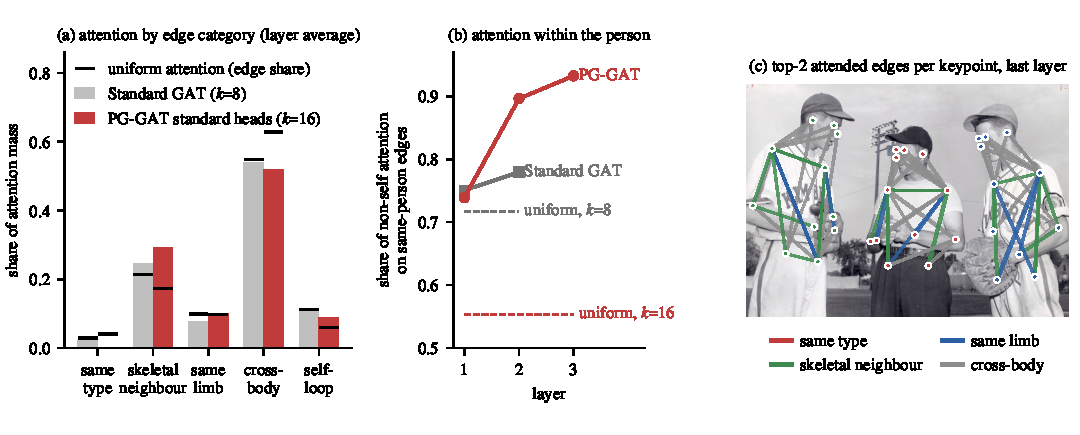
\includegraphics[width=\textwidth]{figures/attention_edges.pdf}
    \caption{Attention of the standard GATv2 baseline and of PG-GAT's standard heads over the 1\,248 multi-person COCO \texttt{val2017} scenes.
    (a) Share of attention by edge category, averaged over layers;
    black ticks mark the share that uniform attention over the neighbourhood would give.
    (b) Share of attention on edges within the same person, per layer, with the uniform share dashed.
    (c) The two most-attended incoming edges of every keypoint in the final layer on the scene of Figure~\ref{fig:embedding},
    coloured by category.}
    \label{fig:attention}
\end{figure*}

\subsection{What survives synthetic-to-real transfer}
\label{sec:disc_transfer}

% --- from chapter5_transfer.tex 5.2.1-5.2.6 ---
Throughout, synthetic accuracy was a poor predictor of real accuracy.
Exact depth made synthetic grouping almost perfect and real grouping worse; graph partitioning was the best synthetic
head and among the worst on COCO; the hyperbolic embedding matched a Euclidean one of four times its dimension on
synthetic data but not after fine-tuning; and fine-tuning itself, which changes no part of the architecture, yielded a
gain of 0.0705 on COCO, comparable in size to the 0.0738 that the whole architecture sweep added on synthetic data.
Figure~\ref{fig:transfer} plots this pattern across all 27 configurations that carry both measurements.
Synthetic training remains valuable as a controlled setting with exact identities in which architectural ideas can be
isolated, and as the starting representation that fine-tuning then adapts; an improvement measured there counts as
evidence only when the mechanism behind it also makes sense on real keypoints.
The variants of Section~\ref{sec:results_variants} illustrate the point: each introduced structure motivated in
principle, and none produced an advantage at the COCO operating point.

\begin{figure}[!t]
    \centering
    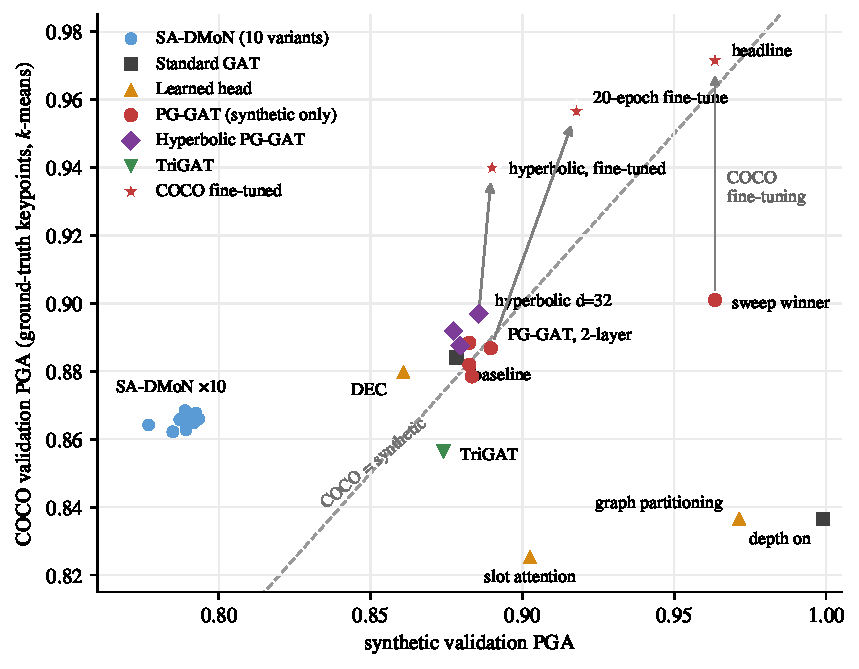
\includegraphics[width=\columnwidth]{figures/transfer_scatter.pdf}
    \caption{Synthetic-validation pose grouping accuracy against COCO-validation pose grouping accuracy on ground-truth keypoints, for the 27 configurations that report both.
    Points below the diagonal lose accuracy in transfer;
    arrows join the synthetic-only models to their COCO fine-tuned versions.}
    \label{fig:transfer}
\end{figure}

\subsection{The cost of modularity and the effective person count}
\label{sec:disc_modularity}

% --- from chapter5_modularity_autonomy.tex 5.3.1-5.3.3; effective-K numbers from results.md per-image dump ---
Separating grouping from detection carries a measured cost.
On matched detections the autonomous pipeline trails the native grouping by 0.0203 to 0.0220 across the three detector
families, and the stability of that difference suggests it belongs to the modular formulation rather than to an
interaction with one detector.
The likely source is information the native mechanisms have and PG-GAT does not: AE tags are learned together with the
detector's features and training distribution, whereas PG-GAT sees only coordinates, visibilities, and joint types.
Nor is modularity bought through a smaller model; PG-GAT has 333\,552 parameters, against about 561 in HigherHRNet's tag
head within a detector of 28.6 million.
What the cost buys is reuse --- the same frozen network groups the output of three different detectors without
retraining, which the native mechanisms, embedded in their own detectors, do not offer.
For a fixed detector whose native grouping is available, the results favour the native grouping; the modular design is
useful where detectors are exchanged, upgraded, or developed independently of the grouping stage.
The system-level measurement sharpens the point: on identical joints the cost is 0.048 AP, concentrated in scenes with
more people than the synthetic training data contained (Section~\ref{sec:results_ap}), and the matched-detection
accuracy therefore understates what a deployed system loses.

The K-head behaves unexpectedly.
Replacing the annotated count with an estimate might be expected to add error, yet on HigherHRNet detections it raises
accuracy by 0.0053 even though it matches the annotated count in only 76.1\,\% of scenes.
The annotated count describes the people in the image, whereas $k$-means operates on the detections that survive; at a
keypoint recall of 79.3\,\%, some annotated people contribute few or no detections, and forcing a cluster for them
splits a well-represented person instead.
The head predicts from the detected embeddings and their number; its mean prediction of 2.46 people sits below the
annotated mean of 2.74.
Measured against the number of distinct annotated people actually present among the matched detections, its exact
agreement rises from 76.0\,\% to 82.1\,\% in a re-run of the evaluation.
The detector swap supports this reading (Figure~\ref{fig:predk}): the advantage of the predicted count grows as recall
falls and reverses sign once the input is complete.
The four points are consistent with an effective-person-count mechanism rather than proof of it, since detector
identity, visibility patterns, and localisation also differ between them.
In a modular pipeline behind an imperfect detector, estimating the count from the detections is therefore not merely a
stand-in for an oracle; the annotated count is not necessarily the right target for the input the grouping stage
actually receives.

\begin{figure}[!t]
    \centering
    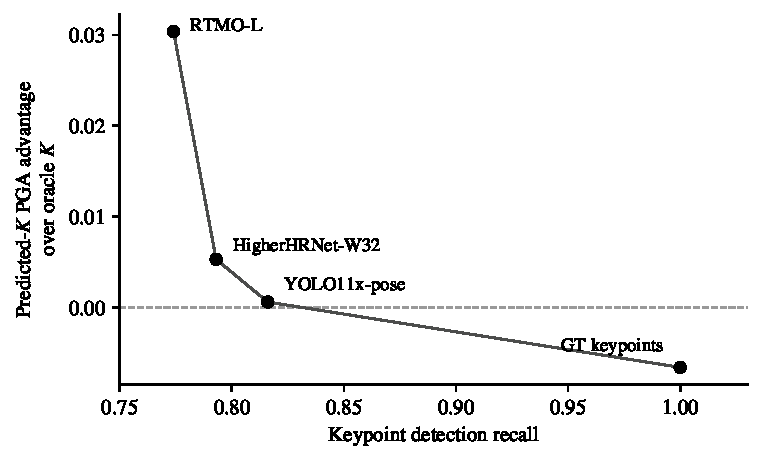
\includegraphics[width=\columnwidth]{figures/predk_recall.pdf}
    \caption{Difference in end-to-end pose grouping accuracy between the predicted and the annotated person count, against keypoint recall, for the three detectors and for ground-truth keypoints.}
    \label{fig:predk}
\end{figure}